\subsection{Digital filtrering} \label{sec:teori_filter}
Der findes to former for digital filtrering; Infinite Impulse Response (IIR) og Finite Impulse Response (FIR). Der ses hertil både fordele og ulemper ved begge filtertyper \citep{blandford2012}.

FIR-filtre kan laves, således de har en lineær fase, og vil altid være stabile. FIR-filtre designes ved at benytte eksempelvis frekvenssampling eller en bestemt vindue-type, hvilket giver en overførselsfunktion. Denne overførselsfunktion kan herved benyttes som et digitalt filter \citep{blandford2012}. 

I modsætning til FIR-filtre, har IIR-filtre ikke en lineær fase, og kan være ustabile. Udover dette har IIR-filtre stejlere sidelobes end et FIR-filter med samme antal koefficienter. Dette betyder, at filteret er mindre hukommelseskrævende og kan arbejde hurtigere. IIR-filtres designprocedure er udledt af den procedure, som de analoge filtre er designet efter. Af denne grund laves IIR-filtre, ligesom analoge filtre, som Butterworth, Chebyshev type 1 og 2 og elliptiske filtre \citep{blandford2012}. Disse er illustreret på \autoref{fig:filtre}.

IIR-filteret består af et forward FIR-filter, der omfatter tælleren, b koefficienter, for nullerne samt et feedback FIR for nævneren, a koefficienterne, for polerne. IIR-filtret udregnes ved anvendelse af følgende formel, der fremgår af \autoref{eq:iirfilt} \citep{francis2009}. 

\begin{equation} \label{eq:iirfilt}
	y(n)= \sum_{i=0}^{n} b_{(i)} \cdot x(n-i)+ \sum^{m}_{i=0} a_{(i)} \cdot y(m-i)
\end{equation}


Hvor $a_{(i)}$ samt  $b_{(i)}$ er IIR-filtrets koefficienter. Kvantiseringen af koefficienterne påvirker frekvens responsen. Nævner koefficienterne samt deres position som poler har en betydning for IIR-fitrets stabilitet\citep{francis2009}.

\begin{figure}[H]
\centering
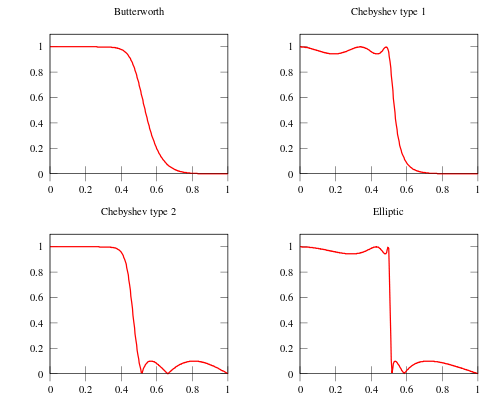
\includegraphics[width=0.8\textwidth]{figures/filtre}
\caption{De fire filtertyper; Butterworth, Chebyshev 1 \& 2 og elliptisk \citep{wikipedia2016}.}
\label{fig:filtre}
\end{figure}

\noindent
Et Butterworth filter er karakteriseret ved ikke at have nogle rippels i hverken pasbåndet eller stopbåndet. Hertil er der, uanset filterorden, en dæmpning på 3 dB ved knækfrekvensen \citep{nilsson2015}.
Et Chebyshev filter har i modsætning til Butterworth et kortere transitionsbånd, som følge af en stejlere dæmpning, dog forekommer der ved et Chebyshev filter enten rippels i pasbåndet eller i stopbåndet. Ved et type 1 Chebyshev filter ses rippels i pasbåndet samt en monotont variation i stopbåndet. For type 2 Chebyshev ses der derimod rippels i stopbåndet og en monotont variation i pasbåndet \citep{nilsson2015}. 
Ved det elliptiske filter ses en endnu stejlere dæmpning og dermed et kortere transitionsbånd end ved Butterworth samt Chebyshev filtre. Ved dette filter ses der dog både rippels i pasbånd og stopbånd \citep{nilsson2015}. 

\vspace{3mm}
\noindent
Et moving average filter er et simpelt lavpas FIR-filter, der oftest anvendes til at udglatte et array af data, der er samplet. Der kan vælges forskellig filterlængde ved implementeringen af filteret. Et moving average filter er et vindue med en bestemt størrelse, der bevæger sig henad et array med ét element ad gangen. Værdien af det midterste element i vinduet vil erstattes med gennemsnitsværdien for de data, der er i hele vinduet. Det midsterste element i vinduen må dog ikke erstattes med gennemsnitsværdien før vinduet har passeret, således alle gennemsnitsværdier er baseret på de originale data. Det er derfor vigtigt at huske på de beregnede gennemsnitværdier. Det fremgår af \autoref{fig:maf} et vindue, der i dette tilfælde har en størrelse på 8. Her tages gennemsnittet af de 8 elementer i vinduet, hvorefter denne værdi erstatter værdien på den 4. plads i vinduet.\citep{atmel2002}

\begin{figure} [H]
\centering
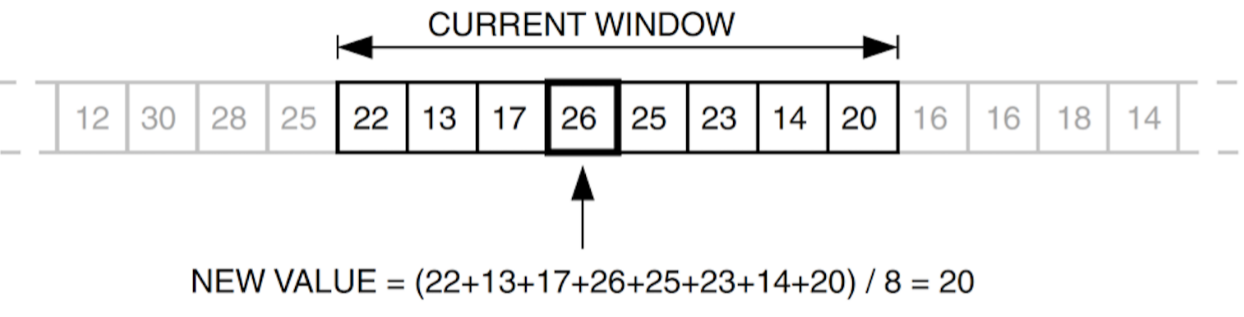
\includegraphics[width=0.8\textwidth]{figures/maf}
\caption{Gennemsnitsværdien beregnes for et vindue for et moving average filter \citep{atmel2002}.}
\label{fig:maf}
\end{figure} 

\noindent
Af \autoref{eq:mafl} fremgår formlen for udregningen af et moving average filter. 
\begin{equation}
	y[i]=\dfrac{1}{M}\sum^{M-1}_{j=0} x[i-j]
\label{eq:mafl}
\end{equation}

\subsubsection{Filtrering af EMG-signal} \label{sec:lavpas_krav}
Under pilotforsøget i \autoref{sec:pilotforsoeg} kunne det ses, at udglatningen af signalet fra det analoge envelopefilter ikke er tilstrækkeligt i forhold til, at signalet skal få et exoskelet til at bevæge sig efter en ALS-patients ben. Da der derfor ønskes at frafiltrere yderligere højfrekvent støj fra det forstærkede, ensrettede og lavpasfiltrerede EMG-signal, vil et IIR-lavpasfilter være fordelagtigt at implementere, da et FIR-filter kan være for tungt for mikrokontrolleren at arbejde med. Dette andet, og digitale, lavpasfilter skal fungere som endnu et envelopefilter, så signalet bliver yderligere udglattet, men skal stadig følge muskelsignalet under øvelsen.
Af denne grund testes forskellige filterdesigns på resultaterne fra pilotforsøget. Dette indebærer, at forskellige knækfrekvenser og filterordener undersøges for at teste, hvordan disse valg påvirker signalet. På denne måde bliver det muligt at beslutte, hvordan filteret skal designes, og hvilke krav der skal opstilles. Filtrene designes som Butterworth-konfigurationer, da der ønskes maksimal fladhed i både pas-, transistions- og stopbåndet og ingen rippels i pas- og stopbåndet, da dette vil påvirke signalet.

Først vælges filterets knækfrevkens ved at afprøve flere forskellige. Eksempler på disse knækfrekvenser ses på \autoref{fig:lp_knaek}, hvor $2~Hz$, $5~Hz$ og $10~Hz$ er repræsenteret. 

\begin{figure} [H]
\centering
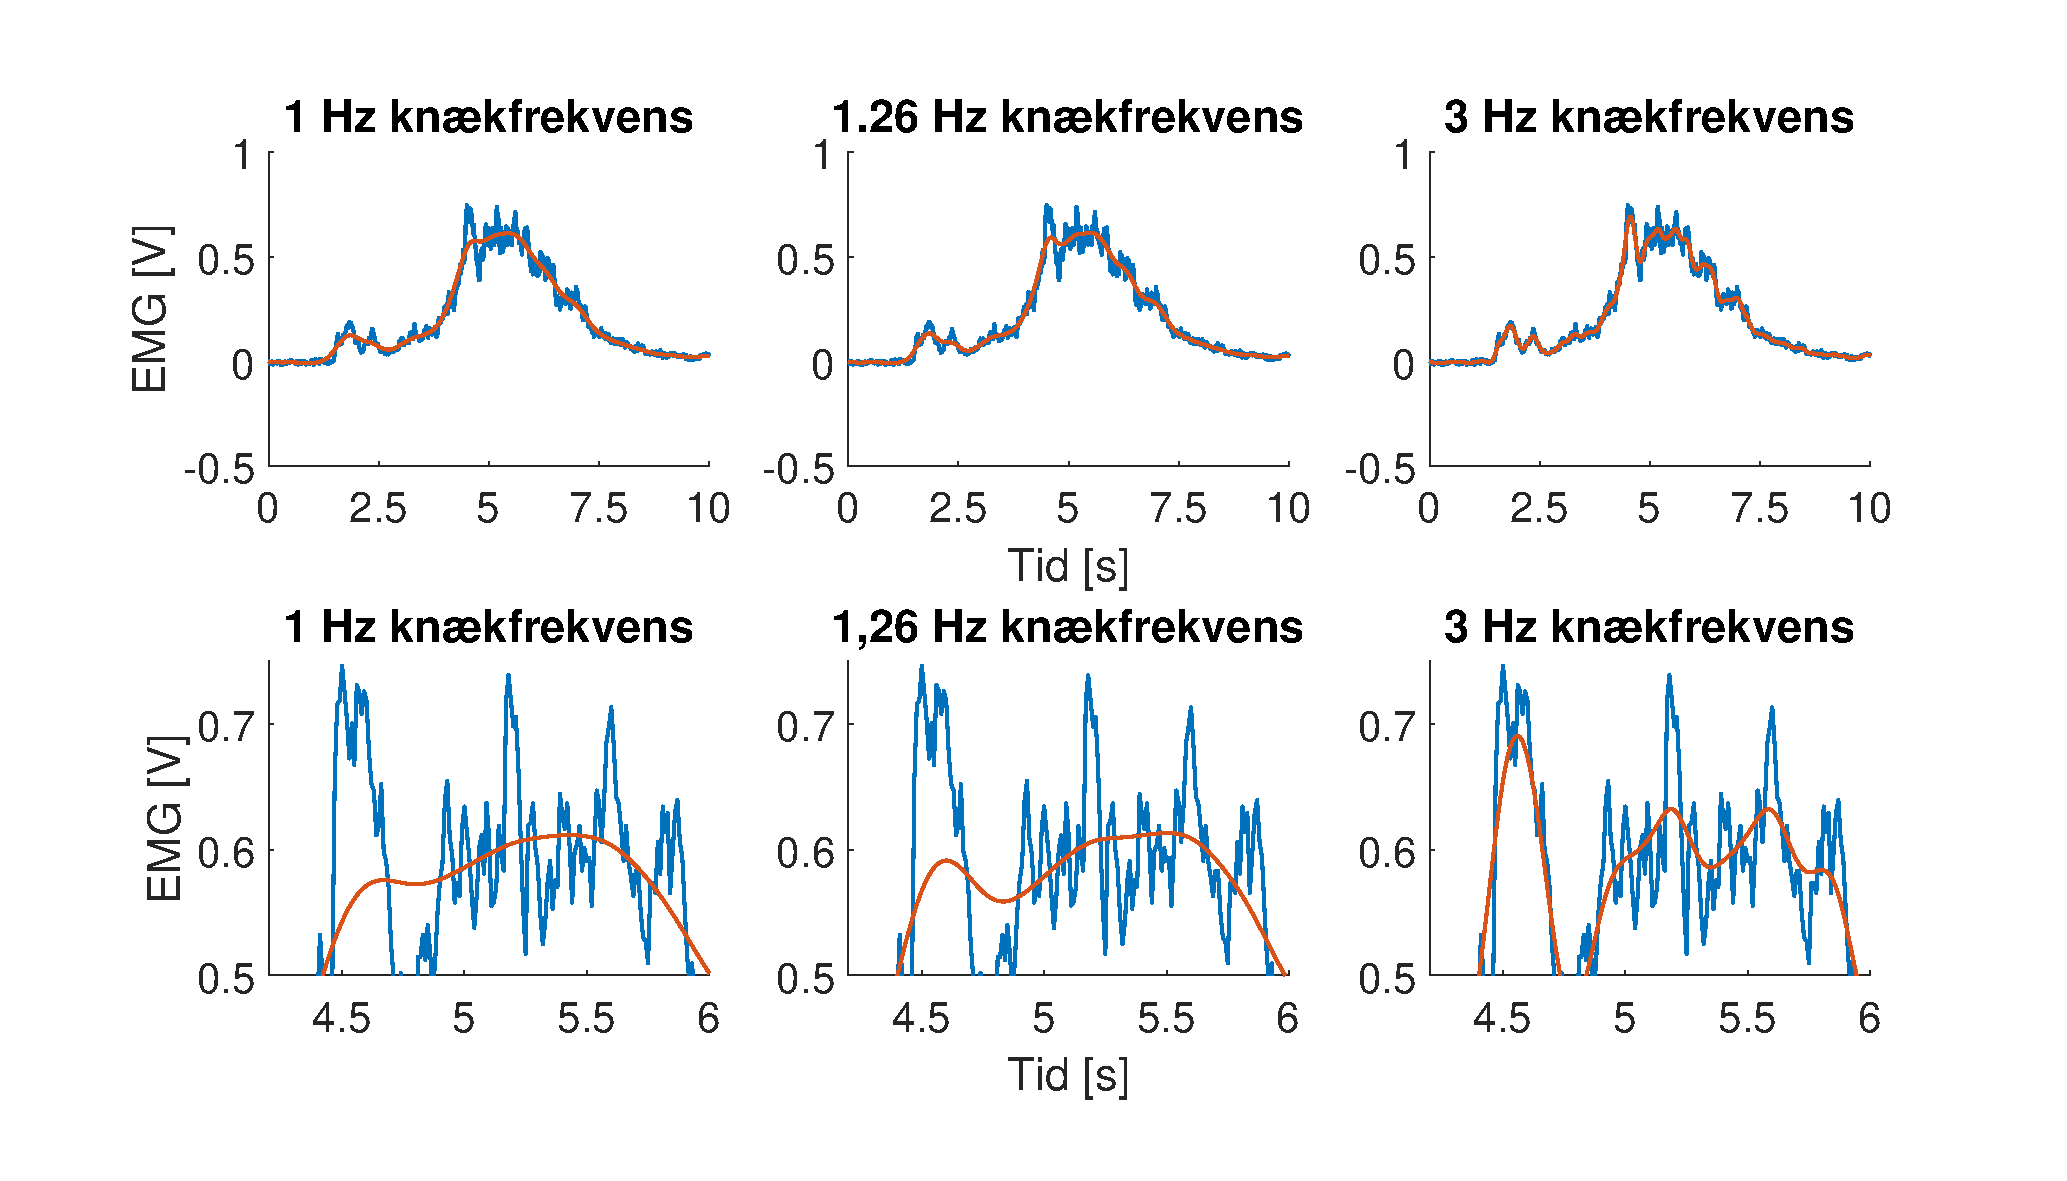
\includegraphics[width=1.0\textwidth]{figures/problemloesning/lavpas_knaek.pdf}
\caption{Øverst ses graferne, hvor de blå linjer på graferne viser resultater fra pilotforsøget. De røde linjer på hver graf viser lavpas IIR-filtre med knækfrekvenser på henholdsvis 2, 5 og $10~Hz$. Nederst ses et udsnit af samme grafer for at illustere filterets påvirkning på signalet.}
\label{fig:lp_knaek}
\end{figure} 

\noindent
Ud fra \ref{fig:lp_knaek} vælges en knækfrekvens på $5~Hz$, da filteret med denne knækfrekvens udglatter spikes og små svingninger i EMG-signalet, der vil kunne forstyrre signalet til exoskelettet. Samtidigt følger filteret signalet, som det kan ses på udsnittene nederst på \ref{fig:lp_knaek}, hvilket de to andre knækfrekvenser ikke formår at gøre.

Herefter bestemmes, på samme måde som ved knækfrekvensen, hvilken filterorden der vil være mest optimal til filteret. 

\begin{figure} [H]
\centering
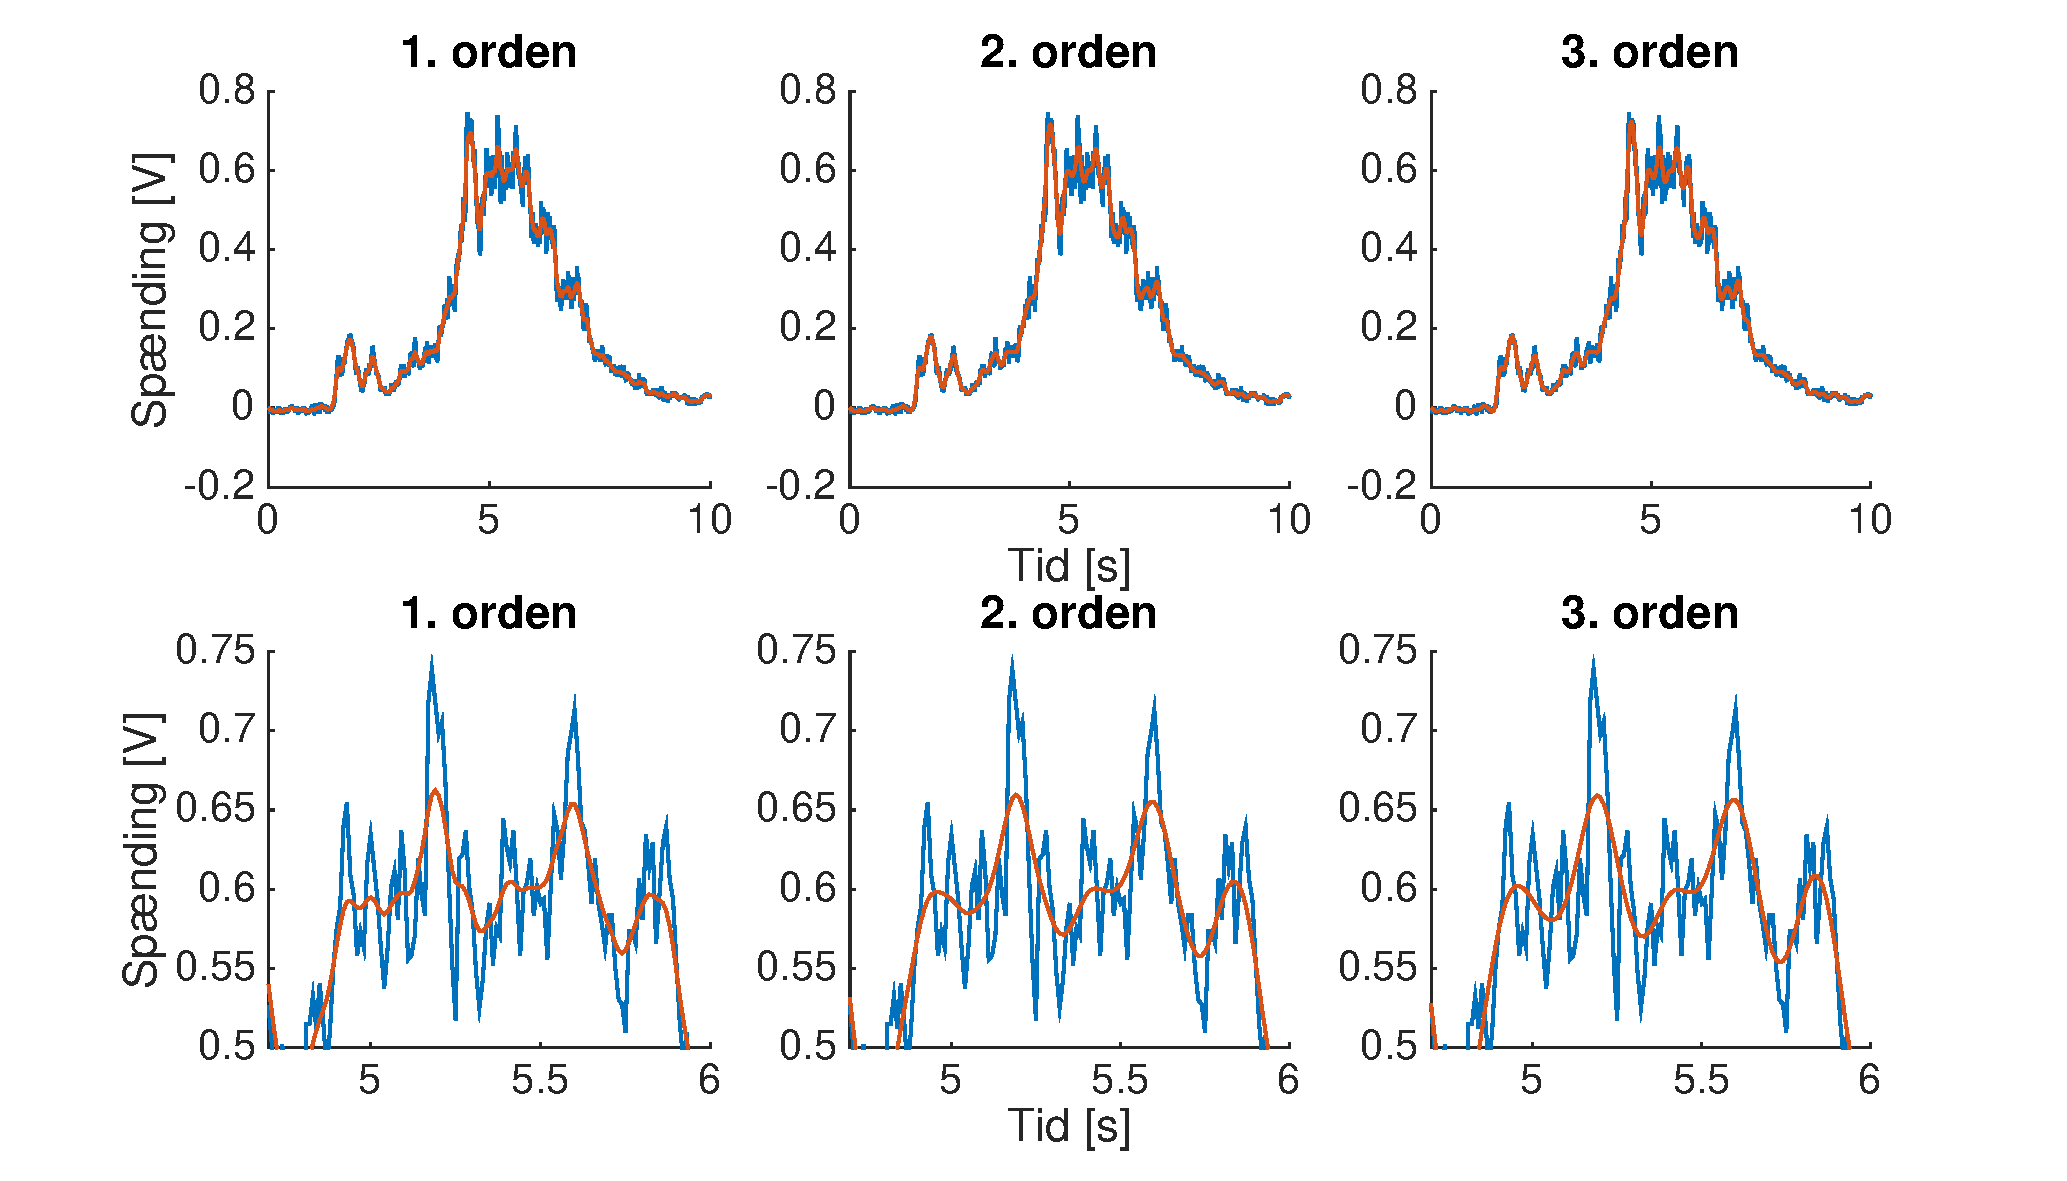
\includegraphics[width=1.0\textwidth]{figures/problemloesning/lavpas_orden.pdf}
\caption{Øverst ses graferne, hvor de blå linjer på grafen viser resultater fra pilotforsøget. De røde linjer på hver graf viser lavpas IIR-filtre med ordner på henholdsvis 1, 2 og 3. Nederst ses et udsnit af samme grafer for at synliggøre, hvilken påvirkning de forskellige ordner har på signalet.}
\label{fig:lp_orden}
\end{figure} 

\noindent
Ud fra \ref{fig:lp_orden} vælges en filterorden på 2, da denne vurderes til være tilstrækkelig. Der ses ingen større forskel i outputsignalet fra filteret, hvis filterordenen hæves yderligere. Dertil vurderes det, at en filterorden på 1 ikke er tilstrækkelig, da dette filters outputsignal afviger mest fra inputsignalet. 

\vspace{3mm}

\textbf{Krav:}
\begin{itemize}
\item Skal følge inputsignalet mest muligt  
\item Skal udformes som et Butterworth lavpasfilter
\item Skal have en knækfrekvens på $5~Hz$
\item Skal have en filterorden på 2
\end{itemize}

\subsubsection{Filtrering af accelerometer-signaler} \label{sec:mavg_krav}
Ud fra accelerometer målingerne i pilotforsøget i \autoref{sec:pilotforsoeg}, vælges det at anvende et moving average filter. Dette forventes at give en mere anvendelig repræsentation af vinklen for det givede accelerometer. Ud fra \autoref{fig:mavgfilter} vælges en filterlængde på 10, da det vurderes, at dette giver en acceptabel forsinkelse af det filtrerede signal uden at påvirke signalet yderligere. Herudover vurderes det at være en passende filterlængde, da det filtrerede signal repræsenterer signalerne fra pilotforsøget i højere grad sammenlignet med de andre filterlængder. Ved implementeringen af et moving average filter opstår der en forsinkelse, der svarer til filterlængden. Denne forsinkelse fremgår af \autoref{fig:mavgfilter}, hvor der ses et udslag i starten, der medfører denne forsinkelse. 

\begin{figure} [H]
\centering
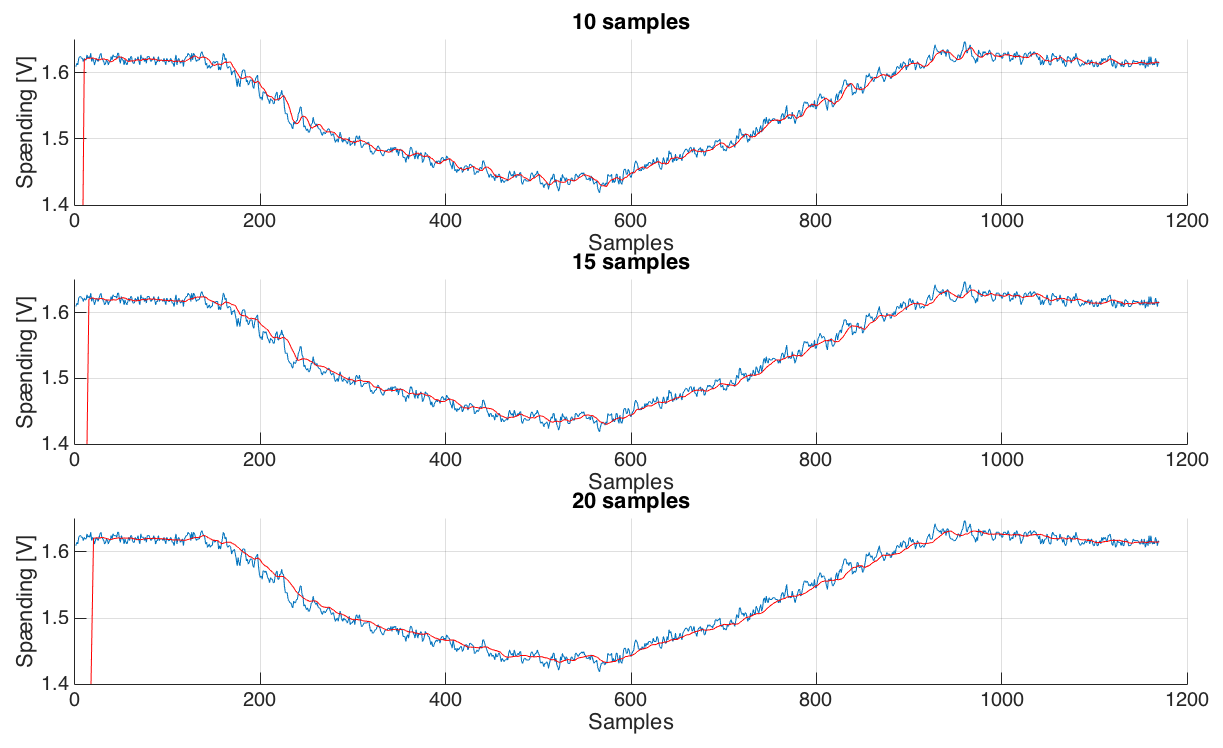
\includegraphics[width=1\textwidth]{figures/problemloesning/mavgfilter_matlab} 
\caption{De blå linjer på grafen viser resultater fra pilotforsøget. De røde linjer på hver graf viser et moving average filter med filterlængde på henholdsvis 10, 15 og 20 samples. I starten af grafen ses et udslag, der svarer til forsinkelsen, som dannes på grund af det implementerede moving average filter. Denne forsinkelse er svarende til filterlængden.}
\label{fig:mavgfilter}
\end{figure}

\vspace{3mm}

\textbf{Krav:}
\begin{itemize}
\item Skal muliggøre en repræsentation af spændinger 
\item Skal have en filterlængde på $10$ samples
\end{itemize}